

\documentclass{article}
\usepackage{graphicx} % Required for inserting images
\usepackage{amsmath}
\usepackage{matlab-prettifier}

\title{Project Part 3: Kalman Filter Development}
\author{Devin Smith \\ UIN: 330000494}
\date{Applied Kalman Filtering\\AERO 689-603}

\begin{document}

\maketitle

\section{Problem Statement}
Begin the development of the Kalman Filter of the continuous-time dynamics of the falling body with discrete-time measurement rage. Recall the mathematical models for the one-dimensional tracking problem form Part 1, illustrated in Figure 1. The tracking problem simulation is shown in Figure 2.

\begin{figure}[h]
    \centering
    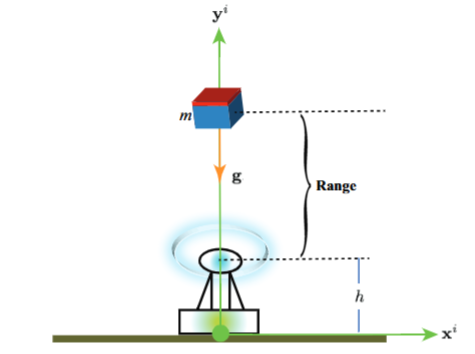
\includegraphics[width=1\linewidth]{Figure_1.png}
    \caption{One-Dimensional tracking problem scenario}
    \label{fig:enter-label}
\end{figure}

\begin{figure}[h]
    \centering
    \includegraphics[width=1\linewidth]{Figure_2.png}
    \caption{Simulation tracking diagram}
    \label{fig:enter-label}
\end{figure}

\subsection{Assumptions}

\begin{enumerate}
    \item Gravity, \textbf{$g$}, and height, \textit{$h$} are known constants
    \item Atmospheric drag is neglected
    \item Motion is one-dimentional (along the \textbf{$y^i$} axis)
    \item Range measurements (measured from the radar antennae dish - not the ground) are available at discrete times
\end{enumerate}

\subsection{Tasks}

\begin{enumerate}
    \item Using the environment and sensor developed in Parts 1 and 2, integrate the Kalman filter into the simulation to generate and process the discrete-time range measurements. Be sure to adequately comment your code.
    \item The inputs of the simulation are
    \begin{itemize}
        \item Initial state, $x_0 = \begin{bmatrix}
            \underline{r}_0 \\ \underline{v}_0
        \end{bmatrix}$
        \item Process noise $Q_s = \begin{bmatrix} 0 & 0 & 0 & 0 \\ 0 & 0 & 0 & 0 \\ 0 & 0 & 0 & 0 \\ 0 & 0 & 0 & q_s 
        \end{bmatrix}$
        \item Measurement Noise $R_k$
        \item Measurement update rate $\Delta t_k$
        \item Height above the ground $h$
        \item Initial state estimation error covariance matrix $P_0$
    \end{itemize}
    \item Consider the following values: $r_0 = \begin{bmatrix}
        0 \\ 1000
    \end{bmatrix} m$, $v_0 = \begin{bmatrix}
        0 \\ 0
    \end{bmatrix} m/s^2$, $h = 2$ m, $q_s = 0.01$ $m^2/s^5$, $\Delta t_k = 0.5$ s, $R_k = 4$ $m^2$, and $P_0 = 
    \begin{bmatrix} 0 & 0 & 0 & 0 \\ 0 & 100 & 0 & 0 \\ 0 & 0 & 0 & 0 \\ 0 & 0 & 0 & 10 
    \end{bmatrix}$
\end{enumerate}

\section{Problem Formulation}

\subsection{Continuous-Time Model}
Recall the continuous-time state-space mathematical equations derived in part 1 of the one-dimensional tracking problem.

\subsubsection{Dynamics}

\begin{equation}
    \underline{\dot{r}}(t) = \underline{v}(t)
\end{equation}
\begin{equation}
    \underline{\ddot{r}}(t) = \underline{\dot{v}}(t) = -\underline{g}
\end{equation}

\begin{equation}
    \underline{\dot{x}}(t) = \mathbf{F}(t)\underline{x}(t) + \mathbf{G}(t)\underline{u}(t) + \underline{w}(t)
\end{equation}

\begin{equation*}
    \begin{bmatrix} \dot{r_x}(t) \\ \dot{r_y}(t) \\ \dot{v_x}(t) \\ \dot{v_y}(t) \end{bmatrix} = 
    \begin{bmatrix} 0 & 0 & 1 & 0 \\ 0 & 0 & 0 & 1 \\ 0 & 0 & 0 & 0 \\ 0 & 0 & 0 & 0 \end{bmatrix}
    \begin{bmatrix} r_x(t)\\r_y(t)\\v_x(t)\\v_y(t) \end{bmatrix} +
    \begin{bmatrix} 0 & 0 \\ 0 & 0 \\ 0 & 0 \\ 0 & 1 \end{bmatrix}
    \begin{bmatrix} 0\\-g \end{bmatrix} +
    \begin{bmatrix}
        0 \\ 0 \\ 0 \\ w(t)
    \end{bmatrix}
\end{equation*}

\begin{equation*}
    E\{\underline{w}(t)\} = \underline{0}
\end{equation*}
\begin{equation*}
    E\{\underline{w}(t)\underline{w}(\tau)^T\} = \mathbf{Q}_s(t)\delta(t-\tau), \forall t,\tau
\end{equation*}
\begin{equation*}
    \mathbf{Q}_s = 
    \begin{bmatrix} 0 & 0 & 0 & 0 \\ 0 & 0 & 0 & 0 \\ 0 & 0 & 0 & 0 \\ 0 & 0 & 0 & q_s \end{bmatrix}
\end{equation*}

\begin{equation*}
    \underline{x}_0 = \begin{bmatrix}
            \underline{r}_0 \\ \underline{v}_0
        \end{bmatrix}
\end{equation*}

\subsection{Discrete-Time Model}
Recall the discrete-time state-space mathematical equations derived in part 1 of the one-dimensional tracking problem.

\subsubsection{Dynamics}

\begin{equation}
    \underline{x}_k = \boldsymbol{\phi}_\mathrm{k-1}\underline{x}_\mathrm{k-1} + \underline{u}_\mathrm{k-1} + \underline{w}_\mathrm{k-1}
\end{equation}

\begin{equation}
    \boldsymbol{\phi}(t_k,t_\mathrm{k-1}) = e^{\mathbf{F}(t_k - t_\mathrm{k-1})}
\end{equation}

\begin{equation}
    \underline{u}_\mathrm{k-1} = \int_{t_\mathrm{k-1}}^{t_k} \boldsymbol{\phi}(t_k, \tau)\mathbf{G}(\tau)\underline{u}(\tau)d\tau
\end{equation}

\begin{equation*}
    \begin{bmatrix} 0 \\ r_k \\ 0 \\ v_k \end{bmatrix} = 
    \begin{bmatrix}
        1 & 0 & \Delta t & 0\\
        0 & 1 & 0 & \Delta t \\
        0 & 0 & 1 & 0 \\
        0 & 0 & 0 & 1
    \end{bmatrix}
    \begin{bmatrix} 0\\r_\mathrm{k-1}\\0\\v_\mathrm{k-1} \end{bmatrix} - g
    \begin{bmatrix}
        0 \\
        \dfrac{{\Delta t}^2}{2} \\
        0 \\
        \Delta t
    \end{bmatrix}
    +
    \underline{w}_\mathrm{k-1}
\end{equation*}

\begin{equation}
    \underline{w}_\mathrm{k-1} = \int_{t_\mathrm{k-1}}^{t_k} \boldsymbol{\phi}(t_k, \tau)\underline{w}(\tau)d\tau
\end{equation}

\begin{equation}
    E\{\underline{w}_\mathrm{k-1}\} = \int_{t_\mathrm{k-1}}^{t_k} \boldsymbol{\phi}(t_k, \tau)E\{\underline{w}(\tau)\}d\tau = \underline{0}
\end{equation}

\begin{equation}
    E\{\underline{w}_\mathrm{k-1}\underline{w}_\mathrm{k-1}^T\} = \mathbf{Q}_\mathrm{k-1} = 
    \int_{t_\mathrm{k-1}}^{t_k} \boldsymbol{\phi}(t_k, \tau)\mathbf{Q}_s(\tau)\boldsymbol{\phi}^T(t_k, \tau)d\tau
\end{equation}

\begin{equation*}
    \mathbf{Q}_\mathrm{k-1} = q_s
    \begin{bmatrix}
        0 & 0 & 0 & 0\\
        0 & \dfrac{{\Delta t}^3}{3} & 0 & \dfrac{{\Delta t}^2}{2} \\
        0 & 0 & 0 & 0 \\
        0 & \dfrac{{\Delta t}^2}{2} & 0 & \Delta t
    \end{bmatrix}
\end{equation*}

\subsubsection{Measurements}

\begin{equation}
    \underline{y}_k = \underline{r}_k + \underline{b}
\end{equation}

\begin{equation}
    \underline{y}_k = \mathbf{H}\underline{x}_k + \underline{b} + \underline{v}_k
\end{equation}

\begin{equation*}
    y_k = 
    \begin{bmatrix}
        0 & 1 & 0 & 0
    \end{bmatrix}
    \begin{bmatrix} r_{x_k} \\r_{y_k} \\v_{x_k} \\v_{y_k} \end{bmatrix} - h + \nu_k
\end{equation*}

\begin{equation*}
    E\{\nu_k\} = 0
\end{equation*}

\begin{equation*}
    E\{\nu_k \nu_j\} = R_k\delta_kj
\end{equation*}

\subsection{Kalman Filter}
In order to initialize the Kalman filter, there must be an initial estimate, $\hat{x}_0$, and error covariance matrix, $P_0$. The matrix $P_0$ is an input for the simulation, and it is used to generate an initial error, $e_0$. The initial estimate $\hat{x}_0$ is then calculated via Equation 12.

\begin{equation}
    \hat{x}_0 = x_0 + e_0
\end{equation}

Starting with these initial estimation parameters, the state transition matrix, the discretized control input, and the discretized process noise covariance, the estimated state and estimation error covariance matrix can be propagated forward using Equations 13 and 14. 

\begin{equation}
    \hat{x}_k^-=\phi_{k-1}\hat{x}_{k-1}^++u_{k-1}
\end{equation}

\begin{equation}
    P_k^-=\phi_{k-1}P_{k-1}^+\phi_{k-1}^T+Q_{k-1}
\end{equation}

Note that in these equations, the $-$ superscript denotes an \textit{apriori} value while the $+$ superscript denotes an \textit{aposteriori} value for a given discrete point in time. Once the state has been propigated to determine the apriori values, the Kalman gain is calculated via Equation 15.

\begin{equation}
    K_k = P_k^-H_k^T(H_kP_k^-H_k^T+R_k)^{-1}
\end{equation}

With the Kalman gain calculated, the aposteriori values for the state estimate and the error covariance matrix are calculated via Equations 16 and 17.

\begin{equation}
    \hat{x}_k^+=\hat{x}_k^-+K_k(y_k-H_k\hat{x}_k^-)
\end{equation}

\begin{equation}
    P_k^+=(I-K_kH_k)P_k^-
\end{equation}


\section{Simulation}
\subsection{Process}
Using the simulation diagram in Figure 2 and the desired user inputs from section 1.2, a simulation of the environment was created in MATLAB. This simulation contains several functions which take in the user inputs and simulate the falling object with process and measurement noise. The structure of the simulation is as follows:

\begin{enumerate}
    \item User inputs are defined.
    \item Generate a discrete-time state-space model of the dynamics (using a simulation time step). Generate a discrete-time state-space model of the measurements and dynamics (using the measurement sampling rate).
    \item Initialize the states, process noise, measurement noise, and radar measurement at $t=0$.
    \item Initialize the apriori state estimate and error covariance, the Kalman gain, and the aposteriori state estimate and error covariance at $t=0$.
    \item Simulate the environment until the object falls below the radar dish.
    \begin{itemize}
        \item Generate process noise and map discretized dynamics forward.
        \item Generate measurement noise and discretely measure range.
        \item Propagate state estimates and error covariance forward, calculate Kalman gain, and update state estimate and error covariance.
        \item Check if object is below radar.
    \end{itemize}
    \item Plot the states, measurements, process noise, measurement noise, range estimates, and state estimate errors.
\end{enumerate}

\subsection{Results}
The results of the simulation with defined user inputs in section 1.2 are shown in Figures 3-12.

\begin{figure}[h]
    \centering
    \includegraphics[width=.8\linewidth]{env_pos.png}
    \caption{True position vs time}
    \label{fig:enter-label}
\end{figure}

\begin{figure}[h]
    \centering
    \includegraphics[width=.8\linewidth]{env_vel.png}
    \caption{True velocity vs time}
    \label{fig:enter-label}
\end{figure}

\begin{figure}[h]
    \centering
    \includegraphics[width=.8\linewidth]{env_om.png}
    \caption{Process noise vs time}
    \label{fig:enter-label}
\end{figure}

\begin{figure}[h]
    \centering
    \includegraphics[width=.8\linewidth]{env_range.png}
    \caption{Range measurements vs time}
    \label{fig:enter-label}
\end{figure}

\begin{figure}[h]
    \centering
    \includegraphics[width=.8\linewidth]{env_nu.png}
    \caption{Measurement noise vs time}
    \label{fig:enter-label}
\end{figure}

\begin{figure}[h]
    \centering
    \includegraphics[width=.8\linewidth]{kf_range.png}
    \caption{Range estimate vs time}
    \label{fig:enter-label}
\end{figure}

\begin{figure}[h]
    \centering
    \includegraphics[width=.8\linewidth]{kf_pos.png}
    \caption{Y-position estimate error vs time (apriori)}
    \label{fig:enter-label}
\end{figure}

\begin{figure}[h]
    \centering
    \includegraphics[width=.8\linewidth]{kf_vel.png}
    \caption{Y-position estimate error vs time (aposteriori)}
    \label{fig:enter-label}
\end{figure}

\clearpage
\subsection{Discussion}
As more measurements were taken, the state estimate errors eventually reduced to smaller values, with their standard deviations eventually reaching a steady state. Regarding at the range values for this simulation, the outliers from the measurements can be seen to have an effect on the position errors, however, the Kalman filter reduces the effects of these outliers. 
\section{Summary}

Under the assumptions described in Section 1.1, the one-dimensional tracking model can be represented with both continuous-time and discrete-time state-space models of the dynamics, as well as a discrete-time model of the measurements. Equations 1-11 contain the equations for the continuous-time and discrete-time models. Using Figure 2 and the desired user inputs, a simulation was made for the environment of the dynamics and measurements, as well as the Kalman filter. Figures 3-7 showcase the results of the simulation for the given numerical values for the problem in Section 1.2.
\par
With these mathematical models, the linear dynamics and measurements can be simulated with process and measurement noise. Additionally, a Kalman filter was used to process the measurements and generate state estimates. In later parts of the problem, the models will be modified with two-dimensional motion, and eventually non-linear dynamics and additional filtering methods. 

\end{document}
